\documentclass[letterpaper,11pt]{article}
\oddsidemargin -1.0cm \textwidth 17.5cm

\usepackage[utf8]{inputenc}
\usepackage[activeacute,spanish]{babel}
\usepackage{amsfonts,setspace}
\usepackage{amsmath}
\usepackage{amssymb, amsmath, amsthm}
\usepackage{comment}
\usepackage{float}
\usepackage{amssymb}
\usepackage{dsfont}
\usepackage{anysize}
\usepackage{multicol}
\usepackage{enumerate}
\usepackage{graphicx}
\usepackage[left=1.5cm,top=1.5cm,right=1.5cm, bottom=1.7cm]{geometry}
\setlength\headheight{1.5em} 
\usepackage{fancyhdr}
\usepackage{multicol}
\usepackage{hyperref}
\usepackage{wrapfig}
\usepackage{subcaption}
\pagestyle{fancy}
\fancyhf{}
\renewcommand{\labelenumi}{\normalsize\bfseries P\arabic{enumi}.}
\renewcommand{\labelenumii}{\normalsize\bfseries (\alph{enumii})}
\renewcommand{\labelenumiii}{\normalsize\bfseries \roman{enumiii})}

\begin{document}

\fancyhead[L]{\itshape{Facultad de Ciencias F\'isicas y Matem\'aticas}}
\fancyhead[R]{\itshape{Universidad de Chile}}

\begin{minipage}{11.5cm}
    \begin{flushleft}
        \hspace*{-0.6cm}\textbf{FI1100-6 Introducción a la Física Moderna}\\
        \hspace*{-0.6cm}\textbf{Profesor:} Diego Mardones\\
        \hspace*{-0.6cm}\textbf{Auxiliares:} Gabriel O\textsc{\char13}Ryan, Camila Sepúlveda, Alejandro Silva\\
        \hspace*{-0.6cm}\textbf{Ayudante:} Sebastián Vargas
    \end{flushleft}
\end{minipage}

\begin{picture}(2,3)
    \put(366, 10){
\includegraphics[scale=0.9]{Imágenes/logo/dfi-fcfm.pdf}}
\end{picture}

\begin{center}
	\LARGE\textbf{Auxiliar \# 4:}\\
	\Large{Ondas Propagativas y Estacionarias}
\end{center}

\vspace{-1cm}
\begin{enumerate}\setlength{\itemsep}{0.4cm}

\rfoot[]{pág. \thepage}

\item[]

\item Considere una onda viajera descrita por:
\[ y(x,t) = 5 \cos{(4x-2t)}\]
    \begin{enumerate}
        \item Demuestre que $y(x,t)$ es solución a la ecuación de ondas.
        \item Determine sentido de propagación, velocidad, longitud de onda y periodo.
        \item Determine la velocidad transversal de la cuerda, ¿cuál será su máximo valor?
    \end{enumerate}

\item \textbf{(Propuesto)} Una cuerda  de  masa  $m$  y  largo  $L$  sostiene  un  bloque  de  masa  $M$,  como  se  indica  en la  figura. La distancia entre el extremo fijo y la polea es $l$. El bloque oscila libre de roce hasta un ángulo  máximo  $\theta$.  Determine,  para  un  pulso  que  viaja  a  través  de  la  cuerda  horizontal,  el  tiempo  de  viaje  del  pulso  cuando  el  péndulo  pasa  por  la  parte  más  baja  y  cuando  está  en  el  ángulo  máximo. Compare  los  resultados  e  indique  en  cuál  condición  el  pulso  tarda  menos  tiempo.

\begin{figure}[h!]
    \centering
    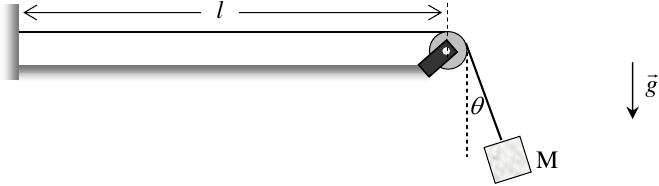
\includegraphics[width = 0.5\linewidth]{Imágenes/aux4/cuerda-pendulo.png}
\end{figure}

\item Demuestre para una cuerda de largo $L$, con densidad lineal $\mu$ y tensión $\tau$ que:
    \begin{enumerate}
        \item si la cuerda posee extremos fijos en $x=0$ y $x=L$, se tiene que:
        \[k_n = \frac{n\pi}{L}, \quad \omega_n = \frac{n\pi}{L}\sqrt{\frac{\tau}{\mu}}\]
        
        \item si la cuerda posee extremos libres en $x=0$ y $x=L$, se tiene que:
        \[k_n = \frac{n\pi}{L}, \quad \omega_n = \frac{n\pi}{L}\sqrt{\frac{\tau}{\mu}}\]
        
        \item si la cuerda posee un extremo fijo en $x=0$ y un extremo libre en $x=L$, se tiene que:
        \[k_n = \frac{\pi(2n-1)}{2L}, \quad \omega_n = \frac{\pi(2n-1)}{2L}\sqrt{\frac{\tau}{\mu}}\]
    \end{enumerate}

\newpage   
\item Una cuerda de guitarra de longitud $L=0.7$ \texttt{m} y densidad lineal de masa $\rho_L = 7 $ \texttt{g/m} emite una nota de frecuencia $f=190$ \texttt{Hz} en su primer modo de oscilación.
    \begin{enumerate}
        \item Determine la longitud de onda del modo fundamental de oscilación.
        \item Calcule la velocidad con que se propagan las ondas en la cuerda.
        \item Determine la tensión de la cuerda.
        \item Calcule la frecuencia de oscilación de los siguientes tres modos de oscilación de la cuerda.
        \item El mástil de la guitarra tiene varios trastes que permiten presionar la cuerda para disminuir la longitud efectiva de la misma. El primero está ubicado a una distancia de $0.04$ \texttt{m} del extremo de la cuerda. ¿Qué frecuencia emite la cuerda en su modo fundamental al presionar sobre este traste?
        \item Se quiere afinar la cuerda para que entregue una nota sol ($f = 196$ \texttt{Hz}) al oscilar en su modo fundamental. ¿Qué tensión se debe dar a la cuerda para lograr afinar la cuerda?
    \end{enumerate}

\end{enumerate}
\end{document}